\chapter{Introducción}
\label{chap:introduccion}

\section{Descripción de la Realidad Problemática}

Actualmente mucha de nuestra calidad de vida es posible gracias a los bosques, estos además son el hogar de más de la mitad de todas las criaturas y organismos de nuestro planeta. Los bosques dan a la humanidad una variedad de regalos que contribuyen en gran medida a nuestra calidad de vida actual \cite{balvanera2012servicios}.


La deforestación es la pérdida de bosques naturales, algunas de las causas que generan este proceso son: La construcción de carreteras, las actividades agrarias, el desarrollo urbano, la minería ilegal \cite{fearnside2005deforestation}, se puede mencionar algunas consecuencias de la deforestación como son: La pérdida de la biodiversidad, la desertización, inundaciones, desaparición de las selvas tropicales, cambio climático, etc. \cite{garcia2016deforestation}.


Según el MINAGRI (Servicio Nacional Forestal y de Fauna Silvestre) y el MINAM (Programa Nacional de Conservación de Bosques para la Mitigación del Cambio Climático) el Perú registró una deforestación de 164,662 hectáreas de bosques amazónicos en el 2016, cifra que representa un incremento del 5.2\% comparado con el año anterior (156,462 hectáreas). La deforestación en el 2016 es la segunda más alta de los últimos 16 años, solo superada por la registrada en el 2014 (177,566 hectáreas) \cite{noticia1}.


Existen distintos sistemas de monitoreo de cambios de bosques con el fin de detectar deforestación a lo largo del mundo \cite{MinisteriodelambientedelPeru}, actualmente MINAM cuenta con un software de rastreo de deforestación a base de imágenes satelitales, pero este utiliza procesos manuales \cite{MinisteriodelAmbiente}.
%
\section{Delimitaciones y Definición del Problema}

\subsection{Delimitaciones}
\begin{enumerate}
    \item Aunque existen gran variedad de tipos de cambios solo se tomarán en cuenta aquellos cambios relacionados a los bosques de la Selva Amazónica Peruana.
    \item El tamaño de las imágenes del análisis será de 256 x 256 con una resolución espacial de 3 metros de la plataforma de Planet.
    \item Se tomará imágenes satelitales ortorectificadas para su estudio.
    \item No se validará la georeferenciación de las imágenes de entrada.
    
\end{enumerate}


\subsection{Definición del Problema}

Los cambios de suelos son una medida importante para medir el progreso de la deforestación proporcionando información para tomar medidas en contra de la deforestación. La detección de cambios automatizada basada en imágenes satelitales es una herramienta usada en el análisis de la deforestación, uno de los motivo por el cual un análisis hecho por humanos es costoso es la cantidad de esfuerzo y tiempo que este requiere \cite{SINGH1989}, además que este análisis es propenso a errores, por ejemplo, como se muestra en la \figureautorefname ~\ref{maap} MAAP (Monitoring of the Andean Amazon Project) posee una metodología que consta de los siguientes pasos: 
\begin{enumerate}
    \item Alertas provistas por software de terceros.
    \item Verificación usando imágenes LandSat.
    \item Se obtienen imágenes de alta resolución  para realizar los análisis correspondientes.
    \item En caso de encontrar nubes se utilizan imágenes radar.
    \item Análisis de los resultados mediante un proceso manual.
    \item Revisar los resultados.
    \item Publicar en la plataforma de \gls{MAAP}.
\end{enumerate}{}
.

\begin{figure}[H]

\centering
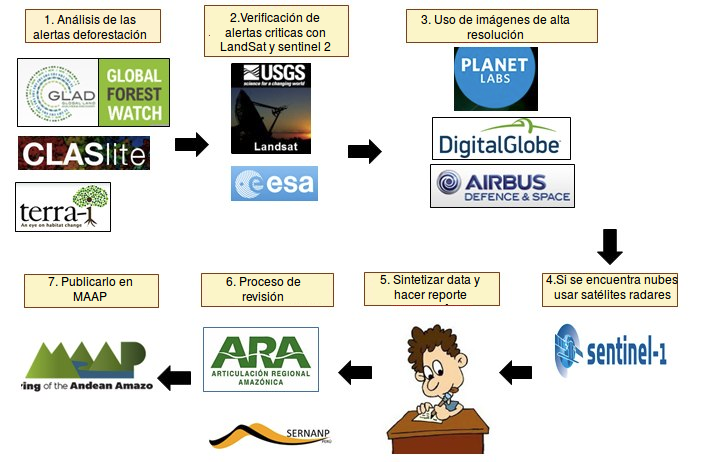
\includegraphics[width=0.8\textwidth]{images/MetologiaMAAPv2.png}
\caption{Metodología de \gls{MAAP} traducida de \cite{AmazonConservation} }
\label{maap}

\end{figure}

Algunos de los sistemas de detección de cambios usados para el análisis forestal en el Perú están basados en imágenes de mediana resolución adquiridas mediante convenio con instituciones extranjeras, al hacer un análisis más detallado de las zonas deforestadas se evidencia que las imágenes de mediana resolución(15 metros) no son suficientes \cite{hansen2013high}.

La detección de cambios en imágenes multitemporales es un problema clásico de la teledetección \cite{Zhu2017}, se han desarrollado varios trabajos que tratan de analizar los cambios con técnicas de procesamiento de imágenes tradicionales\cite{hansen2013high,AlenCastro2015,Anwar2012,Hirschmugl2014,Zhu2014}, sin embargo el uso del aprendizaje profundo aun tiene bastante campo de estudio.













\section{Formulación del Problema}
La detección de cambios realizada manualmente por humanos es una tarea que requiere de mucho esfuerzo y muchas veces esta tarea es susceptible a errores. Aunque existen plataformas de software en Perú que realizan un análisis de deforestación, estas aun presentan procesos manuales.

\section{Objetivo de la Investigación}
\subsection{Objetivo General}
Realizar un modelo computacional para la detección de cambios de la selva amazónica usando imágenes satélites multiespectrales mediante un enfoque de aprendizaje profundo.

\subsection{Objetivos Específicos}
\begin{itemize}[$\circ$]

% \item Estudiar las distintas causas de la deforestación.
  \item Elaborar una base de datos de imágenes satelitales.


 \item Construir un modelo de red neuronal profunda que permita la segmentación semántica de cada imagen.

 \item Elaborar un modelo que permita realizar un mapa de cambios basado en la segmentación semántica. 
    \item Análisis de los resultados.
\end{itemize}

\section{Hipótesis de la Investigación}
Un modelo computacional basado en las redes neuronales profundas será capaz de detectar cambios en imágenes satelitales multitemporales.

\section{Variables e Indicadores}
\subsection{Variable Independiente}
\begin{itemize}
    \item  Cambios planteados por la herramienta MAAP.
    \item  Imágenes Satelitales
    \item Zonas de adquisición.
\end{itemize}

\subsection{Variable Dependiente}
\begin{itemize}
    \item Presencia de cambios(Medio, medio-Alto, Alto): Esto representa que tan grande fue la deforestación en un área determinada.

    \item \textbf{IoU:} este es el método estándar de evaluación, calcula la relación entre la intersección y la unión de dos conjuntos, en segmentación esto es la relación entre nuestro \textbf{ground truth} y nuestra predicción \cite{GarciaGarcia2017}.
    \item \textbf{Accuracy:} Calcula la relación entre el total de pixeles correctamente clasificados y el total de pixeles \cite{GarciaGarcia2017}.
    
\end{itemize}{}

\section{Viabilidad de la Investigación}
\subsection{Viabilidad Técnica}
Como se menciona en \cite{long2015fully} es posible realizar una segmentación semántica mediante redes neuronales convolucionales, y  en el trabajo de \cite{Doshi2018} el uso de redes neuronales convolucionales en la detección de cambios es viable. 

\subsection{Viabilidad Operativa}
El modelo puede ser utilizado por las entidades del estado para la detección de cambios automatizada, sin embargo la propuesta no sera utilizable a gran escala sin una plataforma que gestione las propiedades de las imágenes, el acceso a datos y equipos. El proyecto de \textbf{Sistema de soporte a la toma de decisiones para el manejo forestal, utilizando imágenes satelitales y computación de alto desempeño - IDIBIO-118} propone una plataforma que albergará el proyecto.


\subsection{Viabilidad Económica}
La obtención de las imágenes será mediante la plataforma Planet, esta plataforma da acceso a una cierta cantidad de imágenes gratuitas con fines académicos. Además el proyecto de tesis cuenta con la financiación del proyecto: \textbf{Sistema de soporte a la toma de decisiones para el manejo forestal, utilizando imágenes satelitales y computación de alto desempeño - IDIBIO-118} que financiará los costos asociados




\section{Justificación e Importancia de la Investigación}
\subsection{Justificación}
Se puede entender a la deforestación como el proceso por el cual la superficie forestal es destruida, de esta manera la detección de cambios puede ser usada como un método de detección de deforestación.   

%El cambio de suelos da un indicio de como se da el proceso de deforestación, es por eso que la detección de cambios provee información de soporte para la prevención de la deforestación.

%Encontrar zonas deforestadas puede ser difícil si se trata de realizar mediante una exploración desde el suelo, es por eso que en la actualidad se usan distintas herramientas como imágenes satelitales, fotografías áreas, etc. 

Las imágenes satelitales son de gran ayuda para el análisis de suelos, estas imágenes pueden llegar a zonas donde el acceso es difícil \cite{AlenCastro2015}. El uso de imágenes satelitales es una solución más barata en comparación a la toma de fotografías aéreas, además las imágenes satelitales cuentan con más información que la obtenida mediante la vista humana \cite{unsalan2013multispectral}.


Hace algunos años la adquisición de imágenes satelitales era un problema, actualmente se cuenta con varios repositorios de imágenes libres como son: Earth Obsevation System\footnote{https://eos.com/}, Planet\footnote{https://www.planet.com/} o United States Geological Survey Digital Spectral Library\footnote{https://speclab.cr.usgs.gov/spectral-lib.html}; también existen algunas fuentes de datos libres como las del concurso ``Understanding the Amazon from Space'' de Kaggle\footnote{https://www.kaggle.com/c/planet-understanding-the-amazon-from-space}. 


El Perú adquirió un satélite de alta resolución llamado PeruSat que provee amplia información para los distintos estudios que se deseen realizar, para solicitar imágenes de PeruSat solo es necesario establecer un convenio con CONIDA (Comisión Nacional de Investigación y Desarrollo Aeroespacial).

Las técnicas de aprendizaje profundo han sido usadas en distintas tareas, recientemente se ha comenzado a usar estas técnicas en la teledetección \cite{zhang2016deep} debido a las ventajas que ofrece en problemas de alta dificultad, en cuyos casos no es posible una extracción de características apropiada.

 El aprendizaje profundo es un enfoque en el cual las características no son preprocesadas, el enfoque profundo puede ser útil para el problema de la detección de cambios, dado que se evita este preprocesamiento.
\subsection{Importancia}
La importancia de la investigación radica en que al automatizar el proceso de detección de cambios esta  puede aumentar la velocidad del proceso y lograr un mejor desempeño al momento de tomar las acciones necesarias por parte de las entidades gubernamentales correspondientes.
\section{Limitaciones de la Investigación}
La resolución espacial de las imágenes satelitales y/o la presencia de cultivos y/o pasto en las imágenes satelitales puede llegar a limitar el resultado del modelo. Además se tiene que considerar que la presencia de nubes y neblina limita la correcta visualización de las escenas y además se requiere de equipos de alta capacidad de procesamiento. 
\section{Tipo y Nivel de la Investigación}
\subsection{Tipo de Investigación}
Según \cite{hernandez2010metodologia} el enfoque de la investigación vendría a ser del tipo cuantitativo  debido a que la investigación tiene las siguientes características:
\begin{itemize}
    \item El problema ya esta delimitado.
    \item Se ha realizado la revisión del estado del arte una vez definido el problema.
    \item Se construyó un hipótesis en base a la revisión del estado del arte.
    \item Las imágenes son consideradas como matrices de números.
\end{itemize}{}

\subsection{Nivel de la Investigación}
El nivel de la investigación es exploratoria debido a que se parte de un campo estudiado como las redes neuronales convolucionales y se explora el conocimiento hacia una nueva area como son los modelos de sistema de detección de cambios en Perú.

\section{Método y Diseño de la Investigación}
\subsection{Método de la Investigación}
Como se menciona en ~\cite{long2015fully} el uso de las redes neuronales para la clasificación de imágenes es de bastante importancia desde que el trabajo de~\cite{krizhevsky2012imagenet} en 2012 ganó el concurso Imagenet\footnote{ImageNet es una base de datos de imágenes organizada según la jerarquía de WordNet (actualmente solo los sustantivos), en la que cada nodo de la jerarquía está representado por cientos y miles de imágenes. Actualmente se tiene un promedio de más de quinientas imágenes por nodo.} que consistía en etiquetar imágenes, a partir de eso distintos trabajos comenzaron a hacer el uso de las redes neuronales convolucionales para etiquetado de imágenes y para la detección de objetos.
El próximo paso fue la inferencia de cada pixel, los primeros intentos para la segmentación semántica~\cite{ning2005toward,   ciresan2012deep, farabet2013learning} realizaban una clasificación para cada uno de los pixeles tomando en cuenta una ventana, es decir se utilizaba una red neuronal para cada pixel. Usar una red neuronal para clasificar cada uno de los pixeles es bastante costoso,se menciona que la red propuesta en \cite{krizhevsky2012imagenet}  realiza la tarea de clasificación de una imagen de 224x224 en 1.2 ms mientras que la arquitectura propuesta en \cite{long2015fully} puede generar una grilla de 10x10 de una imagen de 500x500 en 22 ms logrando asi una velocidad 5 veces mayor al de clasificar cada pixel.

\subsection{Diseño de la investigación}
\label{sec:MetodologiaElvis}
La detección de cambios se hará utilizando técnicas de aprendizaje profundo.

La investigación se dividirá en 3 etapas. 
\begin{enumerate}
\item La primera etapa sera la construcción de una base de datos apropiada incluye:
\begin{itemize}
 \item Recolección de imágenes satelitales de distintas fuentes (Kaggle, Planet, PeruSat).
 \item Procesamiento de las imágenes para correcciones geométricas o atmosféricas.
 \item Segmentación manual de las imágenes con su respectivo etiquetado. 
\end{itemize}
\item En la segunda etapa se construirá un modelo de red convolucional para poder realizar un segmentado semántico a cada uno de los pixeles de las imágenes.

%http://lema.rae.es/dpd/srv/search?key=p%EDxel
\begin{figure}[H]
    \centering
    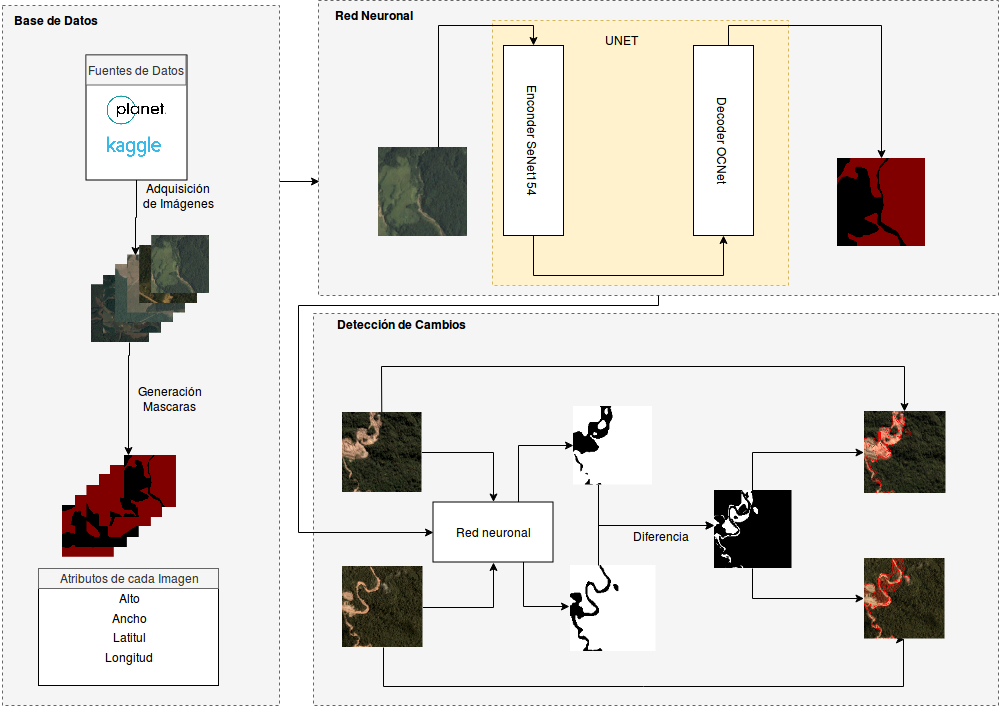
\includegraphics[width=0.8\textwidth]{images/ArquitecturaFinakl.png}
    \caption{Gráfico de la metodología}
    \label{fig:my_label}
\end{figure}
\item En la tercera etapa se seleccionara la mejor configuración de red construir un modelo computacional de detección de cambios basado en el artículo de \cite{doshi2018satellite} para obtener una imagen segmentada.
\end{enumerate}
\section{Técnicas e Instrumentos de Recolección de Información}

\subsection{Técnicas}
Para la obtención de las imágenes satelitales se plantea la búsqueda en la web de repositorios libres de imágenes, además de utilizar el sistema de descargas de imágenes oficiales de la página de Planet\footnote{www.planet.com}. 


\subsection{Instrumentos}
Se usarán frameworks de desarrollo que habilitarán la construcción de las redes neuronales profundas como pueden ser \textbf{Pytorch\footnote{https://pytorch.org/}, Tensorflow \footnote{https://www.tensorflow.org/} o Caffe\footnote{https://caffe.berkeleyvision.org/}}. Se verificará el estado del arte en concursos de segmentación semántica. Para la generación de máscaras se usará herramientas de etiquetado como es \textbf{Labelme\footnote{https://github.com/wkentaro/labelme}}.

\section{Organización del trabajo}
A continuación y a modo de guía de la lectura del documento, se describe la estructura de la tesis y los contenidos esenciales de cada capítulo.
En el capítulo \ref{chap:introduccion} (\textit{Introducción}) se especifica el planteamiento del problema, las variables dependiente e independiente, los objetivos, así como la metodología empleada, y la organización de la tesis. En el capítulo \ref{chap:marcoTeorico}(\textit{Marco Teórico:}) se desarrollarán los conceptos necesarios para poder entender la propuesta. En el capítulo \ref{chap:imagenes}(\textit{Base de datos de Imágenes Satelitales}) se detallará el proceso de construcción de la base de datos. capítulo \ref{chap:desarrollo}(\textit{Desarrollo}) se detalla el proceso de construcción del modelo propuesto. En el capítulo \ref{chap:pruebas} (\textit{Pruebas y resultados}) se describen las pruebas realizadas, los diferentes parámetros que se utilizaron, así como la validación de los resultados, la precisión. En el capítulo \ref{chap:conclusiones} (\textit{Conclusiones y trabajos futuros}): se dan las conclusiones finales de todo el trabajo realizado y se presentan líneas de trabajo que quedan abiertas a futuras investigaciones.

